\begin{tikzpicture}
\draw (0,0) -- node[midway, below] {$ \dfrac{1}{T} $} (2.2,0);

\draw (0,0) -- (75:2.69);

\draw (0.3,0) arc (0:75:0.3) node[midway, right] {$ \ang{75} $};

\draw (2.2,0) -- +(120:3) node[midway,right] {$ \omega_n $};

\draw (1.9,0) arc (180:120:0.3) node[midway, left, yshift=2pt] {$ \theta $};

\draw (0.7,2.6) +(-0.13,-0.48) arc (255:300:0.5) node[coordinate, name=B] {};

\draw[->] (B) +(-0.2,0.1) parabola bend (1,2.4) (1.2,2.5) node[above] {$ \dfrac{\ang{180}-\theta}{2}-\dfrac{\phi}{2}=\ang{45} $};
\end{tikzpicture}